\documentclass{article}
%%%%%%%%%%%%%%%%%%%%%%%%%%%
% Packages
%%%%%%%%%%%%%%%%%%%%%%%%%%%
\usepackage{hyperref}
\hypersetup{
  pdfauthor={Marco Arieli Herrera-Valdez},
  pdftitle={}
  pdftex,
  colorlinks=true,
  urlcolor=Bittersweet,
  linkcolor=blue,
  pdftoolbar=true,
  pdfmenubar=true,
  citecolor=Purple,
  filecolor=blue, 
}
%\usepackage{authblk}
\usepackage{python}
\usepackage{mathtools,amsfonts,amssymb,amsmath}
\usepackage[dvipsnames,svgnames,hyperref,table]{xcolor}
\usepackage{graphicx}
\usepackage{microtype}
\usepackage{sidecap}
%\hypersetup{pdfpagemode=FullScreen}
%\usepackage[left=2.5cm,right=2.5cm,top=0cm,bottom=2cm,includehead]{geometry}
\usepackage{fancyhdr}
%\pagestyle{fancyplain}
%\pagestyle{plain}
\usepackage{lscape}
\usepackage{setspace} 
%\setstretch{1.1}
%\doublespacing
%\usepackage[spanish,es-nodecimaldot]{babel}
\usepackage[utf8]{inputenc}
%\usepackage[latin1]{inputenc}
%\usepackage[applemac]{inputenc}

%% Only if the base font of the document is to be different, say sans serif
% Text layout
\usepackage[T1]{fontenc}
\usepackage[scaled=0.92]{helvet}
\renewcommand*\familydefault{\sfdefault}
%\topmargin 0.0cm
%\oddsidemargin 0.5cm
%\evensidemargin 0.5cm
%\textwidth 16cm 
%\textheight 21cm
% The color packages must appear before the pdfpages package
%\usepackage{chemarr}
\usepackage{listings}
%\usepackage[normalem]{ulem}
%\usepackage[usenames,svgnames,dvipsnames]{xcolor}
%\usepackage[dvipsnames,svgnames,usenames]{xcolor}
%\usepackage{booktabs} % Top and bottom rules for table
\usepackage[font=small,labelfont=bf]{caption} 
%\usepackage{wrapfig}
%\usepackage{subfigure}
%\usepackage{beamerthemesplit}
\usepackage{multirow}
\usepackage{multicol}
\usepackage{longtable}
\usepackage{times}
\usepackage{animate}
\usepackage{pdfpages}
\usepackage{url}
%\usepackage{multimedia}
%\usepackage{movie15} 
%\usepackage{media9} 
\usepackage{verbatim}
%\usepackage{pgflibraryarrows} 
%\usepackage{pgflibraryshapes}
\usepackage{tikz}
%\usetikzlibrary{arrows,shapes,matrix,chains,calc,positioning} 
%\usetikzlibrary{trees,mindmap} 
\usepackage{ifthen}
\usepackage{animate}

% To get the envelope in the author list
\usepackage[misc]{ifsym}
%\usepackage[misc,geometry]{ifsym}

%\Letter after the name of the corresponding author

% --------------------------------------
% Bibliography
% --------------------------------------
%\usepackage[sort&compress]{natbib} 
\usepackage[round,sort&compress]{natbib} 
%\usepackage[numbers,sort&compress]{natbib} 
%\bibliographystyle{plainnat}


% ------------------------------------------------
% Abbreviations and other commands
% ------------------------------------------------
\newcommand{\email}{\textrm{\Letter}}
\newcommand{\corrAuthor}{\textrm{\Letter}}
\newcommand{\insp}{{National Institute of Public Health}}
\newcommand{\cisei}{{Center for Research on Infectious Diseases}}
\newcommand{\imate}{{Mathematics Institute}}
\newcommand{\unam}{{National Autonomous University of Mexico}}
\newcommand{\ua}{{University of  Arizona}}
\newcommand{\uprc}{{University of Puerto Rico in Cayey}}
\newcommand{\mbi}{{Mathematical Biosciences Institute}}
\newcommand{\osu}{{Ohio State University}}
\newcommand{\asu}{{Arizona State University}}
\newcommand{\sols}{{School of Life Sciences}}
\newcommand{\smss}{{School of Mathematical Sciences and Statistics}}
\newcommand{\mcmsc}{{Mathematical, Computational, and Modelling Sciences Center}}
\newcommand{\shesc}{School of Human Evolution and Social Change}
%
 \newcommand{\INSP}{{Instituto Nacional de Salud Pública}}
\newcommand{\CISEI}{{Centro de Investigación Sobre Enfermedades Infecciosas}}
\newcommand{\UNAM}{{Universidad Nacional Aut\'onoma de M\'exico}}
\newcommand{\IM}{{Instituto de Matem\'aticas}}
\newcommand{\IF}{{Instituto de F\'isica}}
\newcommand{\FC}{{Facultad de Ciencias}}
\newcommand{\DM}{{Departamento de Matem\'aticas}}
% \newcommand{\ua}{{Universidad de  Arizona}}
% \newcommand{\asu}{{Universidad Estatal de Arizona}}
% \newcommand{\uprc}{{Universidad de Puerto Rico en Cayey}}
% \newcommand{\mbi}{{Instituto de Biociencias Matem\UTF{00C3}\UTF{00A1}ticas}}
% \newcommand{\osu}{{Universidad Estatal de Ohio}}
% ------------------------------------------------
\newcommand{\lrRound}[1]{\left(#1\right)}
\newcommand{\lrSquare}[1]{\left[#1\right]}
\newcommand{\lrSet}[1]{\left\{#1\right\}}
\newcommand{\lrAbs}[1]{\left|#1\right|}
\newcommand{\lrNorm}[1]{\left\|#1\right\|}
\newcommand{\prob}[1]{\mathbf{P}\left\{ #1\right\}}
\newcommand{\eg}{\textit{e.g.}}
\newcommand{\ie}{\textit{i.e.}}
\newcommand{\potassium}{{K$^+$}}
\newcommand{\kalium}{{K$^+$}}
\newcommand{\hydrogen}{{H$^+$}}
\newcommand{\sodium}{{Na$^+$}}
\newcommand{\natrium}{{Na$^+$}}
\newcommand{\calcium}{{Ca$^{2+}$}}
\newcommand{\chloride}{{Cl$^{-}$}}
\newcommand{\magnessium}{{Mg$^{2+}$}}
\newcommand{\concNa}{[Na]}
\newcommand{\concCa}{[Ca]}
\newcommand{\concCl}{[Cl]}
\newcommand{\concK}{[K]}
\newcommand{\felis}{{{$I_{cyc}$}}}
\newcommand{\icyc}{{{$I_{cyc}$}}}
\newcommand{\Avogadro}{N_{\mathrm{A}}}
\newcommand{\absTemp}{\mathrm{T}}
\newcommand{\GasConstant}{\mathrm{R}}
\newcommand{\Faraday}{\mathrm{F}}
\newcommand{\hPlanck}{\mathrm{h}}
\newcommand{\kBoltzmann}{\mathrm{k}}
\newcommand{\kT}{\mathrm{kT}}
\newcommand{\qElementary}{\mathrm{q}}
\newcommand{\hqovertwokT}[1]{\frac{\mathrm{e_0}#1}{2\mathrm{kT}}}
\newcommand{\hqoverkT}[1]{\frac{\mathrm{e_0}#1}{\mathrm{kT}}}
\def\qovertwokT{\mathrm{\frac{e_0}{2kT}}}
\def\qoverkT{\mathrm{\frac{e_0}{kT}}}
\newcommand{\trace}[1]{{\mathrm{Tr}(#1)}}
\newcommand{\tSm}{{\mathrm{Sm}}}
\newcommand{\tSy}{{\mathrm{Sy}}}
\newcommand{\tSt}{{\mathrm{St}}}
\newcommand{\tF}{{\mathrm{F}}}
\newcommand{\tLFP}{{\mathrm{LFP}}}
\newcommand{\tATP}{{\mathrm{ATP}}}
\newcommand{\tADP}{{\mathrm{ADP}}}
\newcommand{\tCaATP}{{\mathrm{CaATP}}}
\newcommand{\tP}{{\mathrm{P}}}
\newcommand{\tNa}{{\mathrm{Na}}}
\newcommand{\tNaK}{{\mathrm{NaK}}}
\newcommand{\tNaKa}{{\mathrm{NaKa}}}
\newcommand{\tNaP}{{\mathrm{NaP}}}
\newcommand{\tNaT}{{\mathrm{NaT}}}
\newcommand{\tNaH}{{\mathrm{NaH}}}
\newcommand{\tNaCa}{{\mathrm{NaCa}}}
\newcommand{\tNaKCl}{{\mathrm{NaKCl}}}
\newcommand{\tKCl}{{\mathrm{KCl}}}
\newcommand{\tCa}{{\mathrm{Ca}}}
\newcommand{\tCl}{{\mathrm{Cl}}}
\newcommand{\tCaL}{{\mathrm{CaL}}}
\newcommand{\tE}{{\mathrm{E}}}
\newcommand{\tI}{{\mathrm{I}}}
\newcommand{\tGlu}{{\mathrm{Glu}}}
\newcommand{\tGABA}{{\mathrm{GABA}}}
\newcommand{\tACh}{{\mathrm{ACh}}}
\newcommand{\tS}{{\mathrm{S}}}
\newcommand{\tSK}{{\mathrm{SK}}}
\newcommand{\tH}{{\mathrm{H}}}
\newcommand{\tK}{{\mathrm{K}}}
\newcommand{\tKaD}{{\mathrm{KaD}}}
\newcommand{\tKD}{{\mathrm{KD}}}
\newcommand{\tL}{{\mathrm{L}}}
\newcommand{\INa}{{I_\mathrm{Na}}}
\newcommand{\INaT}{{I_\mathrm{NaT}}}
\newcommand{\ICa}{{I_{\mathrm{Ca}}}}
\newcommand{\ICaL}{{I_{\mathrm{CaL}}}}
\newcommand{\IKD}{{I_{\mathrm{KD}}}}
\newcommand{\IKaD}{{I_{\mathrm{KaD}}}}
\newcommand{\IK}{{I_{\mathrm{K}}}}
\newcommand{\IAMPA}{{I_{\mathrm{AMPA}}}}
\newcommand{\INMDA}{{I_{\mathrm{NMDA}}}}
\newcommand{\IGABA}{{I_{\mathrm{GABA}}}}
\newcommand{\INaKATP}{{I_{\mathrm{NaK}}}}
\newcommand{\INaK}{{I_{\mathrm{NaK}}}}
\newcommand{\INaKa}{{I_{\mathrm{NaKa}}}}	
\newcommand{\INaCaX}{{I_{\mathrm{NaCa}}}}
\newcommand{\ILeak}{{I_{\mathrm{L}}}}
\newcommand{\stimtop}{{\textit{Top}}}
\newcommand{\stimup}{{\textit{Up}}}
\newcommand{\stimdown}{{\textit{Down}}}
\newcommand{\diffop}[2]{{\partial_{#1} #2}}
%
\newcommand{\splitPage}[4]{
\begin{minipage}{#1\textwidth}
{#2}
\end{minipage}%
\begin{minipage}{#3\textwidth}
{#4}
\end{minipage}
}

\newcommand{\rfig}[1]{{Fig.~\ref{#1}}}
\newcommand{\rtwofigs}[2]{{Figs.~\ref{#1}~and~\ref{#2}}}
\newcommand{\rfigs}[2]{{Figs.~\ref{#1}-\ref{#2}}}
\newcommand{\req}[1]{{Eq.~\eqref{#1}}}
\newcommand{\rtwoeqs}[2]{{Eqs.~\eqref{#1}~and~\eqref{#2}}}
\newcommand{\reqs}[2]{{Eqs.~\eqref{#1}-\eqref{#2}}}
\newcommand{\eqn}[1]{\begin{equation}#1\end{equation}}
\newcommand{\eqna}[1]{\begin{eqnarray}#1\end{eqnarray}}
\newcommand{\smalleq}[1]
{\begin{equation}{\small #1}\end{equation}}
\newcommand{\smalleqna}[1]{ 
  \begin{small} 
    \begin{eqnarray} #1 \end{eqnarray} 
  \end{small}
}
\newcommand{\tinyeqna}[1]{ 
  \begin{tiny} 
    \begin{eqnarray} #1 \end{eqnarray} 
  \end{tiny}
}
% LaTeX beamer
\newcommand{\slide}[1]{\begin{frame}#1\end{frame}}
\newcommand{\from}[1]{{\tiny From #1.}}
\newcommand{\fuente}[1]{{\tiny #1}}
\newcommand{\source}[1]{{\tiny #1}}
\newcommand{\sS}[3]{{{#1}_{#2}^{#3}}}


%%%%%%%%%%%%%%%%%%%%%%%%%%%
% Edits and reviews
%%%%%%%%%%%%%%%%%%%%%%%%%%%
\newcommand{\aquimequede}{
\vspace{1cm} \textcolor{red}
{\textbf{AQUI ME QUEDE}} \\
\vspace{1cm}}
\newcommand{\mahv}[1]{\textcolor{gray}{$^{MAHV:}$}\textcolor{orange}{#1} }




%%%%%%%%%%%%%%%%%%%%%%%%%%%
% Colored sections
%%%%%%%%%%%%%%%%%%%%%%%%%%%
\newcommand{\headcolor}[1]{\textcolor{Bittersweet}{#1}}
\newcommand{\colorsection}[1]{\section*{\headcolor{#1}}}
\newcommand{\colorsubsection}[1]{\subsection*{\headcolor{#1}}}
\newcommand{\colorparagraph}[1]{\paragraph{\headcolor{#1}}}
\definecolor{lightGray}{rgb}{0.92,0.92,0.92}


%%%%%%%%%%%%%%%%%%%%%%%%%%%
% Figure settings and inclusion/exclusion of figures from the compilation
%%%%%%%%%%%%%%%%%%%%%%%%%%%

\newcommand{\figu}[3]{
\begin{figure}{\begin{center}#3\end{center}}\caption{#1}\label{#2}\end{figure}}
\newcommand{\tablFigu}[3]{
\begin{table}\caption{#1}\label{#2}\begin{center}{#3}\end{center}\end{table}}
\newcommand{\smallcaption}[1]{\caption{{\small#1}}}
%\renewcommand{\caption}[1]{\caption{\begin{small}#1\end{small}}}
\usepackage{comment}
%\excludecomment{cond}
\includecomment{cond}
\newcommand{\showfigs}[1]{}
\begin{cond}
\renewcommand{\showfigs}[1]{\begin{center}#1\end{center}}
\end{cond}

% --------------------------------------
% mahvMacros
% --------------------------------------
% For supplements
% --------------------------------------
%\newcommand{\hbAppendixPrefix}{A}
%
%\renewcommand{\thefigure}{\hbAppendixPrefix\arabic{figure}}
%\setcounter{figure}{0}
%\renewcommand{\thetable}{\hbAppendixPrefix\arabic{table}} 
%\setcounter{table}{0}
%\renewcommand{\theequation}{\hbAppendixPrefix\arabic{equation}} 
%\setcounter{equation}{0}


\newenvironment{suppFig}[4]{
  \begin{figure}[h]
    \begin{center}
      {\includegraphics[#4]{#3}} \caption{\small #1} \label{#2}
    \end{center}
  \end{figure}}

\newenvironment{tab}[3]{
\begin{table}
\begin{center}
{#3} \caption{\small #1} \label{#2}
\end{center}
\end{table}}

% Operators
\DeclareMathOperator{\Tr}{Tr}
\newcommand{\re}[1]{ {\mathfrak{Re}} \left( {#1} \right)}
\newcommand{\im}[1]{ {\mathfrak{Im}} \left( {#1} \right)}
% Transpose upperscript
\newcommand{\transp}[1]{#1^{\mathsmaller T}}

% Column vectors. Usage:
% \colvector{a\\b\\c\\d\\e}
\newcommand{\colvector}[1]{\begin{pmatrix}#1\end{pmatrix}} 

% Column vectors. Usage:
% \colvec{5}{a}{b}{c}{d}{e}
\newcount\colveccount
\newcommand*\colvec[1]{
        \global\colveccount#1
        \begin{pmatrix}
        \colvecnext
}
\def\colvecnext#1{
        #1
        \global\advance\colveccount-1
        \ifnum\colveccount>0
                \\
                \expandafter\colvecnext
        \else
                \end{pmatrix}
        \fi
}

% ----------------------------------
% Code listing 
% ----------------------------------
\lstdefinestyle{customPython}{
  language=Python,
  belowcaptionskip=1\baselineskip,
  breaklines=true,
  %frame=L,
  xleftmargin=\parindent,
  showstringspaces=false,
  basicstyle=\footnotesize\ttfamily,
  keywordstyle=\bfseries\color{green!40!black},
  commentstyle=\itshape\color{purple!40!black},
  identifierstyle=\color{blue},
  stringstyle=\color{orange},
}


\usepackage[utf8]{inputenc}
\title{Macroscopic model of postsynaptic current activation considering presynaptic short term synaptic plasticity and postsynaptic activation}

\date{November 2019}


%
\begin{document}
\maketitle


\begin{abstract}
    Postsynaptic currents depend on the activation of postsynaptic receptors, which depend on presynaptic release of neurotransmitter. In turn, the total postsynaptic current in response to the activation of synapses from a given presynaptic contact depends on the number of synapses in the contact and the probability of activation of the synapses in the contact. We propose a new mechanistic model that consider both interactions as  explanation of different types of short term synaptic plasticity reported in experiments.
    
    
\end{abstract}

\newpage

\tableofcontents
\newpage
\input{SynapticTransmition.tex}



\section{Short term presynaptic plasticity model}

Assume that the intracellular calcium concentration at the presynaptic terminal follows linear decay dynamics toward a steady state according to
\begin{equation}
        \partial_t c = \frac{c_{\infty}-c}{\tau_c} - k I_{Ca}
        \label{eq:dcdt}
\end{equation}


where $k_c$ ($\mu$M / pC) can be thought of as a rate indicating the impact of the net transmembrane flux of calcium on the intracellular concentration of calcium. As a rule of thumb, the value of $k_c$ should be such that the change in the calcium concentration in a presynaptic terminal after a single action potential could be between 50 and 100  $\mu$M.

Consider synapses in which the probability of activation of the release machinery  depends directly upon binding of calcium, and when unbound, decreases linearly. The dynamics for $r$ can then be
\begin{equation}
   \partial_t r =  \alpha c^n(1-r)-\beta r   \label{eq:dpdt}
\end{equation}

with $\alpha$ in ms$^{-1} \cdot \mu$M$^{-n}$ and $\beta$ in  ms$^{-1}$.
Equation \eqref{eq:dpdt}
can be rewritten as 
\begin{equation}
   \partial_t r = \frac{r_{\infty}(c)-r}{\tau_r(c)} 
\end{equation}
with 
\begin{equation}
    \tau_r(c) = \frac{1}{\alpha c^n + \beta}= \frac{1}{\alpha} \lrRound{\frac{1}{ c^n + \frac{\beta}{\alpha}}} 
\end{equation}
\begin{equation}
r_{\infty}(c) = \frac{c^n}{c^n + \frac{\beta}{\alpha}} 
\label{eq:pInfty}
\end{equation}
The fraction $ \beta/\alpha$ is the calcium concentration at which the steady state for $p$. So let $c_m^n=\beta/\alpha$.
The quantum of released neurotransmiter is proportional to $r$ and the proportion of neurotransmiter ready to be releasable $q$ which is considered as normalized. And whose dynamics is as follow: 

\begin{equation}
\partial_t q =  \frac{q_{\infty}-q}{\tau_q} - r q  \label{eq:dxdt}
\end{equation}

If the recovery of $r$ is fast enough, let $r \approx r_{\infty}(c)$, them the system can be reduced to a 2-d system where dynamic of $r$ is $r_{\infty}(c)$.
The system \eqref{eq:dcdt}-\eqref{eq:dpdt}
\begin{eqnarray}
\partial_t c &=& \frac{c_{\infty}-c}{\tau_c} - k I_{Ca}
\\
\partial_t q &=&  \frac{q_{\infty}-q}{\tau_q} -  r_{\infty}(c) q
\end{eqnarray}
Where $c,r,q$ represent the calcium intracellular concentration, an activation variable of neurotransmitter release and the normalized proportion of neurotransmitter ready to be releasable respectively.
\begin{table}
\begin{tabular}{r r l p{0.75\textwidth}}
Parameter & Value & Units & Description \\
\hline &&&\\
$c_{\infty}$ & 0.050 & $\mu$M & Steady state concentration for intracellular calcium \citep{regehr1995calcium}\\
$q_{\infty}$ & 1.0 & $\mu$M & Steady state for the readily releasable pool\\
$\beta/\alpha$ & \sim 0.001 & ms & \citep{destexhe1994synthesis}
\\
$c_{m}=\lrRound{\beta/\alpha}^{1/n}$ & 50 & $\mu$M & Half activating calcium concentration \\
$ k $ & 0.1  &  & Impact of the voltage-dependent calcium current on the intracellular calcium so that peaks are about 50 $\mu$M \citep{regehr1995calcium} \\
$\tau_c$ & 30.0 & ms & recovery time constant of intracellular calcium concentration\\
$\tau_q$ & 20.0 & ms & Recovery time constant for the readily releasable pool\\
$n$ & 4 & & \citep{}  \\
\hline &&&\\
\end{tabular}
\end{table}


% ------------------------------------
\subsection{Analysis considering delta pulses to predict asymptotic behaviours}
% ------------------------------------
Assume that calcium current behaves like a delta pulse function: 
\begin{equation}
    I_{Ca}= - k_c \sum_{i=1}^n \delta(t-t_i) 
\end{equation}
then system () is: 
\begin{eqnarray} 
\label{eq : deltap}
\partial_t c &=& \frac{c_{\infty}-c}{\tau_c} + k_c \sum_{i=1}^n \delta(t-t_i) \\
\partial_t q &=&  \frac{q_{\infty}-q}{\tau_q} - r_{\infty}(c) q \\
\partial_t r &=& \frac{r_{\infty}(c) - r}{\tau_r}  
\\
r_{\infty}(c) &=& \frac{c^k}{c^k + \frac{\beta}{\alpha}} 
\label{eq : deltapp}
\end{eqnarray}
Calcium dynamics: $c_{\infty} = 0 , c_0 = c(t_0) = k $
\\
Pulse times: $t_0, t_1, ..., t_n$
\begin{eqnarray*}
c_0 &=& c(t_0) = k
\\
c(t) &=& c_0 e^{-(t-t_0)/\tau_c}
=k e^{-(t-t_0)/\tau_c}, \quad t_0\leq t <t_1
\\
c_1 &=& c(t_1) = k \lrRound{1 + e^{-(t_1-t_0)/\tau_c}}
\\
c(t) &=& c_1 e^{-(t-t_1)/\tau_c}, \quad t_1\leq t <t_2
\\
c_2 &=& k+ c_1 e^{-(t_2-t_1)/\tau_c}  
\\
&=& k+ k \lrRound{1 + e^{-(t_1-t_0)/\tau_c}} e^{-(t_2-t_1)/\tau_c} 
\\
&=& k+ k  \lrRound{e^{-(t_2-t_1)/\tau_c}  + e^{-(t_2-t_0)/\tau_c}} 
\\
&=& k \lrRound{1+e^{-(t_2-t_1)/\tau_c}  + e^{-(t_2-t_0)/\tau_c}}
\end{eqnarray*}
Therefore, after the $n$th pulse has arrived,
\begin{eqnarray}
c_n &=& k \lrRound{ 
\sum_{i=0}^{n} e^{-(t_n-t_{i})/\tau_c} 
}
\label{eq:cn}
\\
c(t) &=& c_n e^{-(t-t_n)/\tau_c}, \quad t_n\leq t <t_{n+1}
\label{eq:c(t)tn}
\end{eqnarray}
If pulses are periodic (fixed frequency), with $\delta = t_{i+1}-t_i$, then $t_n - t_0 = n \delta$, and equation~\eqref{eq:cn} transforms into
\begin{eqnarray}
c_n &=& k \lrRound{ 
\sum_{i=0}^{n} e^{-i\delta/\tau_c} 
}
\label{eq:cnPeriodicPulses}
\end{eqnarray}
The quantity $a = e^{-\delta/\tau_c}$ represents the decay factor between pulses for calcium. Then the calcium concentration peak after the $n$th pulse is 
\begin{equation}
c_n=k \lrRound{ 
\sum_{i=0}^{n} a^{i} 
}
= k \lrRound{\frac{1-a^{n+1}}{1-a}}
\label{eq:cAsymptotic}
\end{equation}
For instance, if $\delta=50$ ms and $\tau_c = 10$ ms, then $a=e^{-5}$, which means that there is almost no accumulation of intracellular calcium between pulses at 20 Hz. 

\subsection{Qualitative Analysis of the Autonomous System}

Model \eqref{eq : deltap}-\eqref{eq : deltapp} is a kind of non autonomus differential equation with a finite number of time-dependent moments (delta pulses). Between each delta pulse, the model can be interpreted as a continuous autonomus system which is topologically equivalent to each other defined on different  between pulses  interval. Each of these autonomus systems has the form: 
\begin{eqnarray} 
\partial_t c &=& \frac{c_{\infty}-c}{\tau_c} \\
\partial_t q &=& q \frac{q_{\infty}-q}{\tau_q} - r_{\infty}(c) q 
\end{eqnarray}
whose nullclines are easily calculated:
\begin{eqnarray} 
c &=& c_{\infty}\\
q &=& q_{\infty}-\tau_q r_{\infty}(c) \hspace{1cm} and\\
q &=& 0
\end{eqnarray}
and whose equilibrium points also are easily calculated to be $(0,0)$ and  $(0,x_{\infty})$.
The Jacobian matrix can be expressed as 
\begin{eqnarray}
J[f] &=& \begin{pmatrix}-\frac{1}{\tau_c} & 0 \\
p'(c_a)q & \frac{x_{\infty}-2q}{\tau_q}-r_{\infty}(c_a)
\end{pmatrix}
\end{eqnarray}
so that is possible to known the stability at each point if equilibrium which just depend on the values of parameters  $\tau_c$ and $\tau_q$.
Evaluating the Jacobian matrix at the fixed point $(0,0)$ we obtain 
\begin{eqnarray}
J_{(0,0)}[f] &=& \begin{pmatrix}-\frac{1}{\tau_c} & 0 \\
0 & \frac{q_{\infty}}{\tau_q}
\end{pmatrix}
\end{eqnarray}
so the fixed point is a saddle. While at the point $(0,q_{\infty})$ Jacobian matrix is: 
\begin{eqnarray}
J_{(0,0)}[f] &=& \begin{pmatrix}-\frac{1}{\tau_c} & 0 \\
0 & -\frac{q_{\infty}}{\tau_q}
\end{pmatrix}
\end{eqnarray}
So in this case the fixed point is ever a stable node. As we can see, there is not bifurcations depending on parameters $\tau_q$ or $\tau_c$ at each autonomous model obtained of \eqref{eq : deltap}-\eqref{eq : deltapp}. 
\begin{figure}
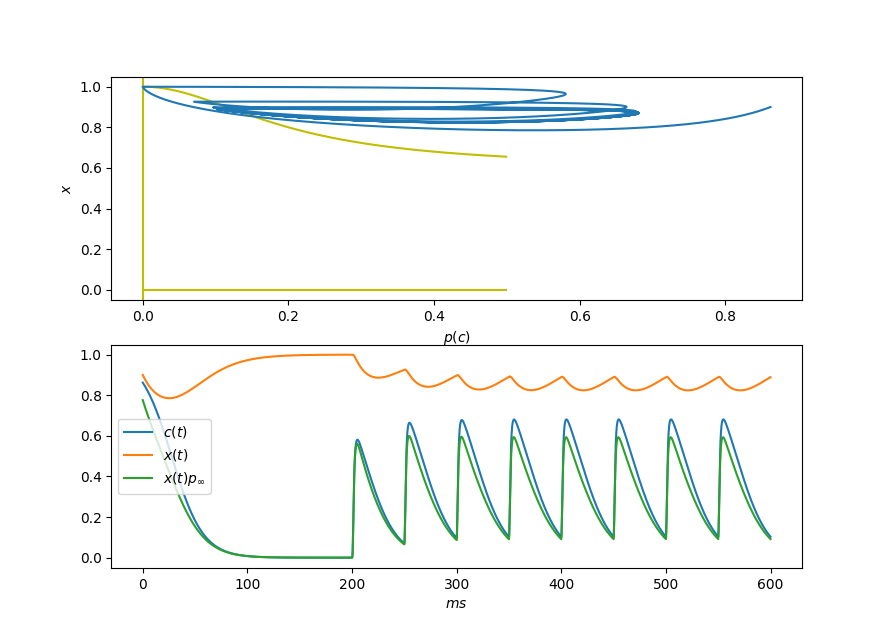
\includegraphics[width=\textwidth]{facilitacion.png}
\caption{phase portrait and temporal courses of a facilitation configuration}
\end{figure}
\begin{figure}
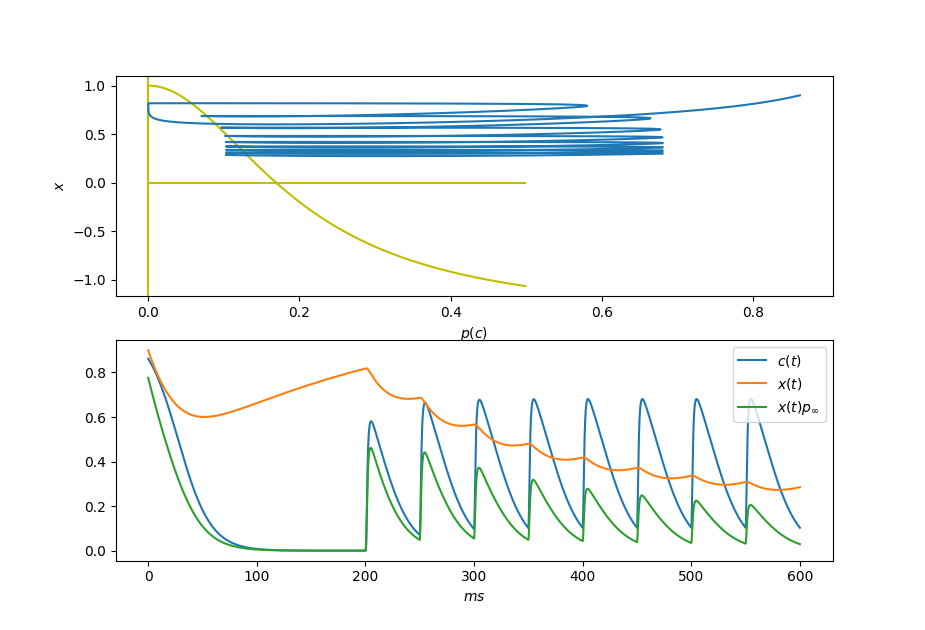
\includegraphics[width=\textwidth]{depression.png}
\caption{phase portrait and temporal courses of a depression configuration}
\end{figure}

%
\newpage


\section{Post synaptic activity due to release of neurotransmitter }

Let it be $p(t)$ the variable of activation of post synaptic currents in a synapse of one synaptic contact which depends on the total of released neurotransmitter. This activation obeys to a lineal dynamic which is given by:

\begin{equation}
\partial_tp = qr\alpha(1-p)-\beta p    
\end{equation}
which can be rewritten as

\begin{equation}
    \partial_tp = \frac{p_{\infty}-p}{\tau_p}
\end{equation}
where 
\begin{equation}
    p_{\infty} = \frac{qr\alpha}{qr\alpha+\beta} 
\end{equation}

and 

\begin{equation}
    \tau_p = \frac{1}{qr\alpha + \beta}
\end{equation}

So the system () is extended to a four dimensional system:

\begin{eqnarray} 
\label{eq : deltap}
\partial_t c &=& \frac{c_{\infty}-c}{\tau_c} + k \sum_{i=1}^n \delta(t-t_i) \\
\partial_t q &=&  \frac{q_{\infty}-q}{\tau_q} - h r q \\
\partial_t r &=& \frac{r_{\infty}(c) - r}{\tau_r}  
\\
\partial_tp &=& \frac{p_{\infty}-p}{\tau_p}
\label{eq : deltapp}
\end{eqnarray}

Using the asymptotic value for $c_n$ (\ref{eq:cAsymptotic}) we can establish a explicit relation between $\tau_c$ and $\tau_r$

\begin{equation}
    \tau_r = \frac{1}{\alpha_r (c_n)^m + \beta_r}
\end{equation} with
\begin{equation}
    c_n = k_c \left(  \frac{1-e^{\frac{-\delta(n+1)}{\tau_c}}}{1-e^{\frac{-\delta}{\tau_c}}}\right)
\end{equation}

So 
\begin{equation}
    \tau_r = \left[ \alpha k_c \left(\frac{1-e^{\frac{-\delta(n+1)}{\tau_c}}}{1-e^{\frac{-\delta}{\tau_c}}}\right)^m - \beta \right]^{-1} 
\end{equation}
So $\tau_r$ depends on $\tau_c$ according to fig().

\begin{figure}
    \centering
    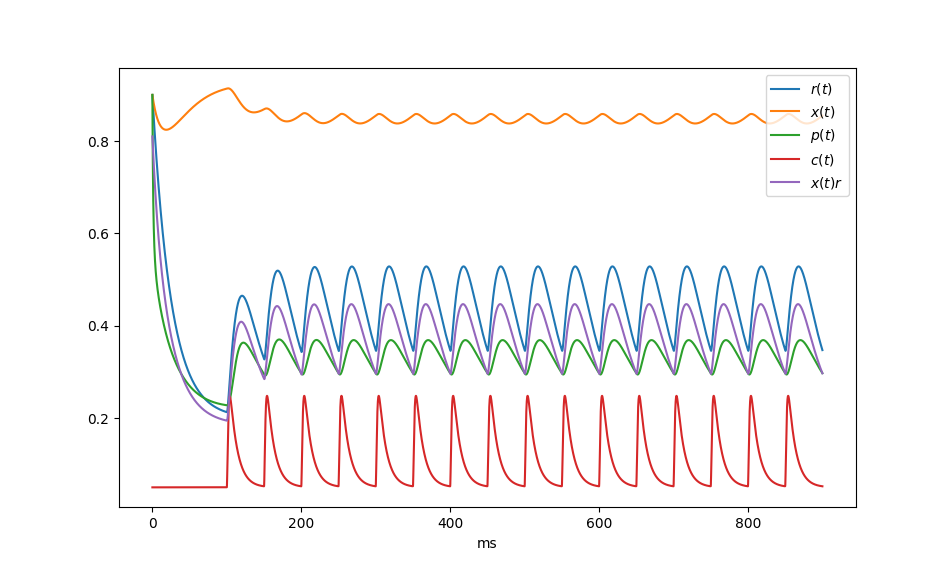
\includegraphics[scale = 0.6]{FacPre_bifPos.png}
    \caption{respuesta bifásica posináptica a pesar de haber facilitación en la liberación de neurotransmisor $xr$}
    \label{fig:my_label}
\end{figure}

\begin{figure}
    \centering
    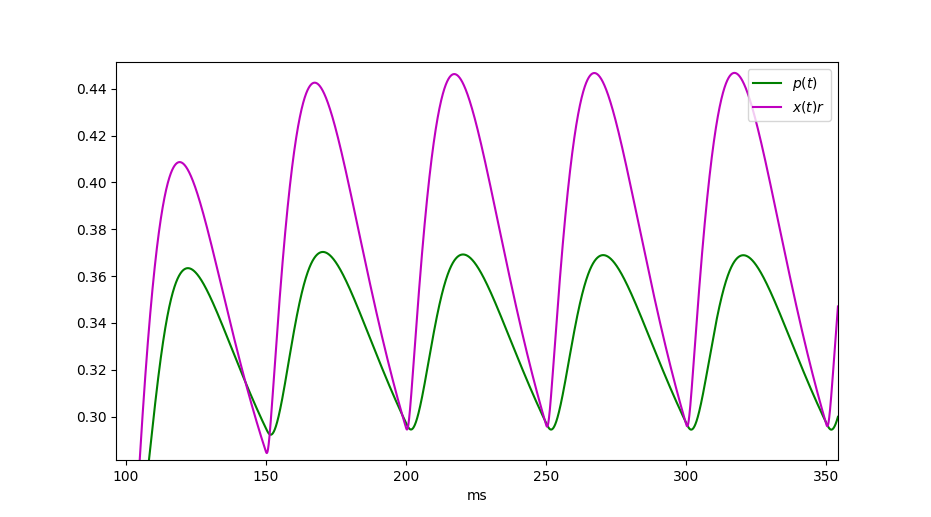
\includegraphics[scale = 0.6]{zoom2.png}
    \caption{zoom de la figura anterior}
    \label{fig:my_label}
\end{figure}

Now, in order to establish a relationship between the rates of recuperation of ready releasable vesicles and the release machinery. We define $L = qr$
Then 
\begin{equation}
    \partial_t L = q \partial_t r + r \partial_t q \\ 
    = q \frac{r_{\infty}(c) - r}{\tau_r} + r \left(\frac{q_{\infty}-q}{\tau_q} - h r q\right)
\end{equation}

The equilibrium state of this variable of release of neurotransmitter give us:  
\begin{equation}
    0 = q \partial_t r + r \partial_t q \\ = q \left(\frac{r_{\infty}(c) - r}{\tau_r}\right) + r \left(\frac{q_{\infty}-q}{\tau_q} - h r q\right)
\end{equation}
which implies that: 
\begin{equation}
     -\frac{r q_{\infty}}{\tau_q}  = q \left(\frac{r_{\infty} - r}{\tau_r} - r( \frac{1}{\tau_q} + h r ) \right)
\end{equation}
So 
\begin{equation}
     q = \frac{-\frac{r q_{\infty}}{\tau_q}}{\left(\frac{r_{\infty} - r}{\tau_r} - r( \frac{1}{\tau_q} + h r ) \right)}  
\end{equation}


\newpage

\paragraph{Discrete and continuous nature of pre- and postsynaptic events. }

Regard one synaptic contact as the collection of all the synapses made by one presynaptic neuron onto a presynaptic neuron of interest. 

Consider a synaptic contact formed by $N$ synapses and assume that  $p$ is the average probability of activation for the synapses in the contact. If the average probability of release in a 

\begin{equation}
    
\end{equation}


Suppose there are $C$ such presynaptic neurons with with $N_1$,...,$N_C$ synapses, respectively.
Assume that the number of vesicles in the RRP at the $k$th synapse from the $j$th neuron is  $n_{jk}$, with $j \in \lrSet{1,...,C}$, $k\in \lrSet{1,...,N_i}$. If after a single action potential from neuron $j$, the probability of release at the $k$th synapse is $p_{jk}$, and vesicles are released independently at each synapse, then the average number of vesicles released at that synapse is $\hat{n}_{jk} = p_{jk} n_{jk}$. The time course of the normalized presynaptic neurotransmitter release is described by the product $q_{jk}(t) p_{jk}(t)$. 
The postsynaptic current at the $jk$-synapse is then
\begin{equation} 
I(v_{jk}, t)= {a}_{jk} q_{jk}(t) p_{jk}(t)  S\lrRound{ \frac{v_{jk}(t)-v_r}{v_T}}
\end{equation}
where  $v_{jk}$is the postsynaptic voltage, $v_r$ is the reversal potential for the postsynaptic current, and $v_T$ is the thermal potential\footnote{$v_T= kT/q$ where $k$ is Boltzmann's constant, $T$ is the absolute temperature,  $q$ is the elementary charge}.  $S$ is a nonlinear function of $v_{jk}$ that describes the electrodiffusive current in the open channel of the activated receptor and $a_{jk}$ is the maximum amplitude of the postsynaptic current in the open channel that can be thought of as the product of the number of postsynaptic receptors and a conversion factor that transforms the normalized amount of neurotransmitter $q_{jk} p_{jk}$, into the proportion of active post-synaptic receptors at the $jk$-synapse.
The peak amplitude of $I(v_{jk})$ causes a change in the postsynaptic potential that propagates and is modified throughout the propagation path. This postsynaptic current is a function of the amount of neurotransmitter released, the proportion of active receptors, and the postsynaptic membrane potential at the postsynaptic membrane.  

Assuming that all the synapses are excitatory and that the postsynaptic neuron is at rest, let $\bar{v}_{jk}$ represent  the peak postsynaptic  potential at an integration site, say, the soma, resulting from the average release of neurotransmitter at the $ij$-synapse and the subsequent activation of the postsynaptic receptors. The peak in the voltage change that results from the average activation of the $j$th synaptic contact is then $\bar{v}_{j}$ which, at best, equals $\sum_{k=1}^{N_j} \bar{v}_{jk}$ when the peaks occur simultaneously at the soma. It is worth recalling that $\bar{v}_{j}$ is only the sum of the average voltage responses from all the synapses of the $j$th contact. 

Assume that there is no noise, that $p_{jk}$, $n_{jk}$, and the $jk$-quanta $q_{jk}$ are constant for $k \in \lrSet{1,...,N_j}$ and $j \in \lrSet{1,...,C}$, and also that the properties of the postsynaptic membrane along the path of propagation do not change for each combination of synaptic activations $jk_1, ..., jk_m$. Under such circumstances, the peak of the total propagated transients $\bar{v}_{jk_1}+...+\bar{v}_{jk_m}$ can only take a finite number of values. However, even in such circumstances and given that a voltage transient can only reach a few millivolts in amplitude, and that the number of different combinations of activated synapses can be very large, then the idea of being able to distinguish discrete values related to the quanta released at the single synapses seems difficult, if not impossible. The quantal nature of the somatic postsynaptic potentials seems even more impossible to occur in consideration of the fact that each combination of synaptic activations is likely to activate voltage-gated channels along the integration path to different extents.





\section{Cortical-Striatal and Thalamus-Striatal synapses}
\begin{figure}[h]
    \centering
    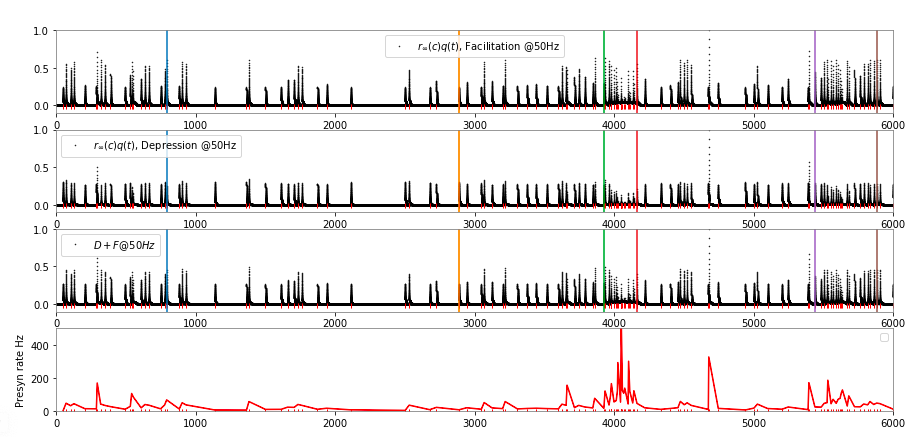
\includegraphics[scale = 0.45]{final.png}
    \caption{Mencionar que este modelo puede ser usado para entender la integración de sinápsis  provenientes simultaneamiente del talamo y corteza}
    \label{fig:my_label}
\end{figure}
\section{Discussion}





\end{document}
